\part{Source}

\chapter{Structure}
\label{source/structure::doc}\label{source/structure:issue}\label{source/structure:structure}
The FVF measurement system is split into various pieces and components.


\section{Pieces}
\label{source/structure:pieces}
The FVF measurement system consists of multiple pieces:
\begin{itemize}
\item {}
Tube

\item {}
Hardware LED controller (Arduino Uno)

\item {}
Client Software

\end{itemize}


\section{Components}
\label{source/structure:components}
The software consists of multiple components written in multiple programming languages:
\begin{itemize}
\item {}
Arduino {\hyperref[source/firmware::doc]{\emph{\emph{Firmware}}}} (C++)

\item {}
LED {\hyperref[source/driver::doc]{\emph{\emph{Driver}}}} (Java)

\item {}
Client {\hyperref[source/software::doc]{\emph{\emph{Software}}}} (Java)

\end{itemize}


\section{Folders}
\label{source/structure:folders}
The folders and what they contain in this repository:
\begin{itemize}
\item {}
\code{docs/} - contains the source files for this documentation

\item {}
\code{driver/} - contains the source files for the {\hyperref[source/driver::doc]{\emph{\emph{Driver}}}}

\item {}
\code{firmware/} - contains the sources files for the {\hyperref[source/firmware::doc]{\emph{\emph{Firmware}}}}

\item {}
\code{software/} - contains the sources files for the {\hyperref[source/software::doc]{\emph{\emph{Software}}}}

\item {}
\code{manual/} - contains the sources files for the manual

\end{itemize}


\chapter{Firmware}
\label{source/firmware:firmware}\label{source/firmware::doc}
The firmware runs on the \textbf{Arduino Uno} board. The board is connected via an Universal Serial Port (USB) to the host computer which runs the measurement software. It's main job is to handle incoming commands (via serial port) and send back feedback notifications.


\section{Available Commands}
\label{source/firmware:available-commands}\begin{itemize}
\item {}
{\hyperref[appendix/led-protocol:protocol-input-on]{\emph{on}}}

\item {}
{\hyperref[appendix/led-protocol:protocol-input-flicker]{\emph{flicker}}}

\item {}
{\hyperref[appendix/led-protocol:protocol-input-off]{\emph{off}}}

\item {}
{\hyperref[appendix/led-protocol:protocol-input-measurement]{\emph{measurement}}}

\item {}
{\hyperref[appendix/led-protocol:protocol-input-ping]{\emph{ping}}}

\end{itemize}

Detailed information about the input and output about the firmware is described in the {\hyperref[appendix/led-protocol::doc]{\emph{\emph{LED Protocol}}}}.


\section{References}
\label{source/firmware:references}\begin{itemize}
\item {}
\href{http://www.arduino.cc/}{Arduino Website}

\item {}
\href{http://www.arduino.cc/en/Main/Software}{Arudino IDE}

\item {}
\href{http://www.arduino.cc/en/Reference/HomePage}{Arduino API}

\end{itemize}


\section{Verification}
\label{source/firmware:arduino-api}\label{source/firmware:verification}
To ensure the flickering frequency a verification measurement has been done with VOLTCRAFT Universal SYSTEM MS-9150 Frequency Counter.

An important Note: The \href{http://www.arduino.cc/en/Reference/Delay}{delay()} method on the Arduino passes the delay in integer values, no floats are possible. For every milliseconds below 16383, \href{http://www.arduino.cc/en/Reference/DelayMicroseconds}{delayMicroseconds()} must be used. The gap happens between 30Hz and 31Hz.


\subsection{Methodology}
\label{source/firmware:methodology}\label{source/firmware:delaymicroseconds}
Voltage has been captured at the pins directly at the measured LED. Each frequency was measured two times and the latter value was used.

Note: Prior sample measurements showed, the value didn't changed after the second measurement for each frequency.

\subsection{Results}
\label{source/firmware:results}

Results are shown in table~\ref{table:firmware-verification}.

\begin{tabularx}{\textwidth}{lll}
\caption{Measurement Results for Flicker-Frequency Accuracy Verification}
\label{table:firmware-verification}
\medskip
\hline
{\bf Frequency} & {\bf Measured Frequency} & {\bf Offset} \\
\hline
\endhead

10Hz
 &
9,996
 &
-0,004
\\

11Hz
 &
11,105
 &
+0,105
\\

12Hz
 &
12,186
 &
+0,185
\\

13Hz
 &
13,146
 &
+0,146
\\

14Hz
 &
14,270
 &
+0,270
\\

15Hz
 &
15,071
 &
+0,071
\\

16Hz
 &
16,110
 &
+0,110
\\

17Hz
 &
17,220
 &
+0,220
\\

18Hz
 &
18,488
 &
+0,488
\\

19Hz
 &
19,200
 &
+0,200
\\

20Hz
 &
19,966
 &
-0,034
\\

21Hz
 &
21,567
 &
+0,567
\\

22Hz
 &
22,678
 &
+0,678
\\

23Hz
 &
23,756
 &
+0,756
\\

24Hz
 &
24,935
 &
+0,935
\\

25Hz
 &
24,941
 &
-0,059
\\

26Hz
 &
26,245
 &
+0,245
\\

27Hz
 &
27,704
 &
+0,704
\\

28Hz
 &
29,191
 &
+1,191
\\

29Hz
 &
29,196
 &
+0,196
\\

30Hz
 &
31,138
 &
+1,138
\\

31Hz
 &
30,772
 &
-0,328
\\

32Hz
 &
31,723
 &
-0,277
\\

33Hz
 &
32,712
 &
-0,288
\\

34Hz
 &
33,702
 &
-0,298
\\

35Hz
 &
34,689
 &
-0,311
\\

36Hz
 &
35,673
 &
-0,327
\\

37Hz
 &
36,657
 &
-0,343
\\

38Hz
 &
37,646
 &
-0,354
\\

39Hz
 &
38,633
 &
-0,367
\\

40Hz
 &
39,621
 &
-0,379
\\

41Hz
 &
40,598
 &
-0,402
\\

42Hz
 &
41,590
 &
-0,41
\\

43Hz
 &
42,578
 &
-0,422
\\

44Hz
 &
43,562
 &
-0,438
\\

45Hz
 &
44,544
 &
-0,456
\\

46Hz
 &
45,275
 &
-0,725
\\

47Hz
 &
46,520
 &
-0,48
\\

48Hz
 &
47,500
 &
-0,5
\\

49Hz
 &
48,481
 &
-0,519
\\

50Hz
 &
49,465
 &
-0,536
\\

51Hz
 &
50,454
 &
-0,546
\\

52Hz
 &
51,436
 &
-0,564
\\

53Hz
 &
52,414
 &
-0,586
\\

54Hz
 &
53,152
 &
-0,848
\\

55Hz
 &
54,389
 &
-0,611
\\

...
 &  & \\

500Hz
 &
468,991
 &
-32,009
\\
\hline
\end{tabularx}


Figure~\ref{fig:firmware-verification} graph shows the scattering of the measured values around the expected linear ideal values.

\begin{figure}[H]
	\centering
	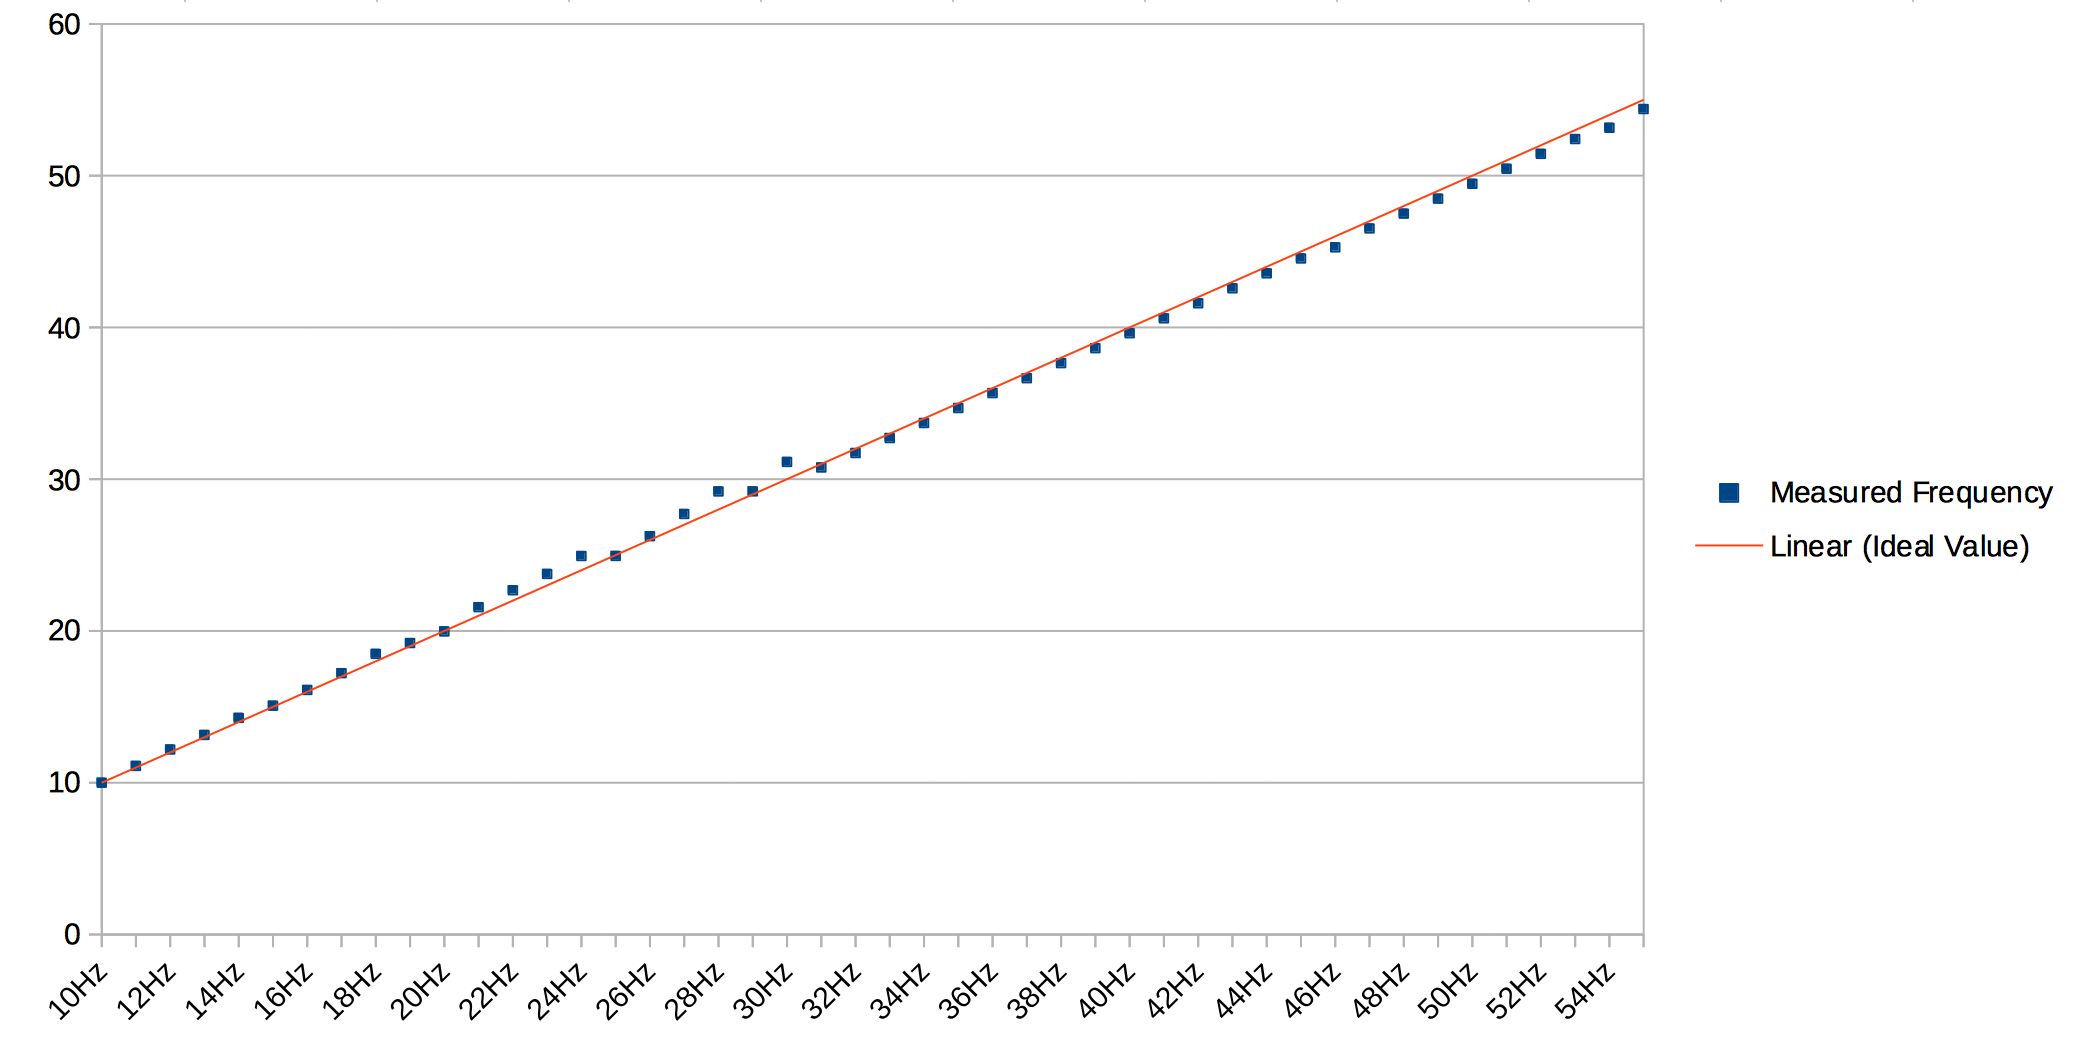
\includegraphics[width=\textwidth]{images/firmware-verification.png}
	\caption{Measurement Results for Flicker-Frequency Accuracy Verification with Frequency Line}
	\label{fig:firmware-verification}
\end{figure}


\chapter{Driver}
\label{source/driver:driver}\label{source/driver::doc}
The LED driver is a Java API to send commands to the {\hyperref[source/firmware::doc]{\emph{\emph{Firmware}}}} and getting notified about feedback from the firmware.


\section{Communication}
\label{source/driver:communication}
The client software talks to the Arduino board through a serial port connection. For this purpose the RXTX interface is used. In order to check whether the connection is still established, the driver periodically sends a ping to the board. Once this connection is interrupted for several reasons, it's assumed the connection is dead.


\section{Protocol}
\label{source/driver:protocol}
The driver implements the {\hyperref[appendix/led-protocol::doc]{\emph{\emph{LED Protocol}}}}.


\section{Deployment}
\label{source/driver:deployment}
The driver is deployed as \code{*.jar} file into the softwares \code{lib/} folder.

\begin{figure}[H]
	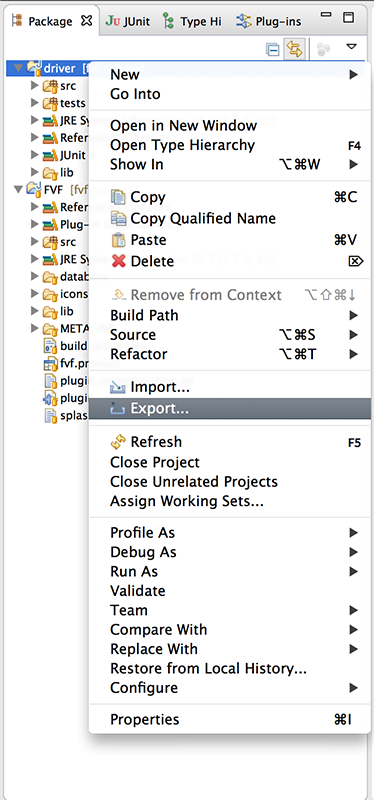
\includegraphics[width=0.45\textwidth]{images/driver_export.png}
	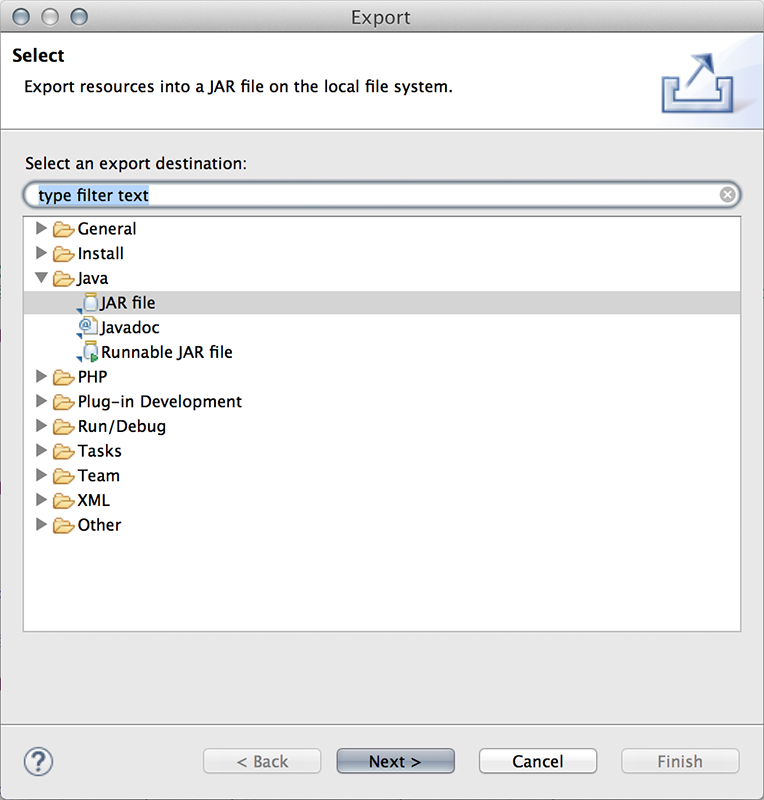
\includegraphics[width=0.45\textwidth]{images/driver_export_dialog.png}
	\caption{Deploy as jar}
	\label{fig:deployment-driver}
\end{figure}

Note: This is not ideal and must be triggered manually. Better solutions are welcome.


\section{Remarks}
\label{source/driver:remarks}
There is a \href{http://rxtx.qbang.org/wiki/index.php/Wrapping\_RXTX\_in\_an\_Eclipse\_Plugin}{rxtx wiki entry} describing how to bundle the jni extension with an eclipse rcp application.


\subsection{Mac OS X}
\label{source/driver:rxtx-wiki-entry}\label{source/driver:mac-os-x}
The normal distributed \code{librxtxSerial.jnilib} is only in 32-bit mode which doesn't match a 64-bit processor architecture and can thus not be autoloaded. See here:

\begin{verbatim}
$ file librxtxSerial.jnilib
librxtxSerial.jnilib: Mach-O universal binary with 2 architectures
librxtxSerial.jnilib (for architecture ppc):  Mach-O dynamically linked shared library ppc
librxtxSerial.jnilib (for architecture i386): Mach-O dynamically linked shared library i386
\end{verbatim}

Luckily there is a 64-bit version available, forged by \href{http://blog.iharder.net/2009/08/18/rxtx-java-6-and-librxtxserial-jnilib-on-intel-mac-os-x/}{Robert Harder}. The eclipse plugin distributes the 64-bit version mentioned here:

\begin{verbatim}
$ file librxtxSerial.jnilib
librxtxSerial.jnilib: Mach-O universal binary with 4 architectures
librxtxSerial.jnilib (for architecture x86_64):       Mach-O 64-bit bundle x86_64
librxtxSerial.jnilib (for architecture i386): Mach-O bundle i386
librxtxSerial.jnilib (for architecture ppc7400):      Mach-O bundle ppc
librxtxSerial.jnilib (for architecture ppc64):        Mach-O 64-bit bundle ppc64
\end{verbatim}


\subsection{Disconnecting}
\label{source/driver:robert-harder}\label{source/driver:disconnecting}
There are some problems between RXTX and properly disconnecting connections. The problems are described in a \href{http://archive.infiniteautomation.com/forum/posts/list/297.page}{forum thread}. The mentioned hacks are implemented precautionally. Probably RXTX version 2.2 should have these issues resolved, yet wasn't available stable at the time of implementation.


\section{References}
\label{source/driver:forum-thread}\label{source/driver:references}\begin{itemize}
\item {}
\href{http://rxtx.qbang.org}{RXTX}

\item {}
\href{http://playground.arduino.cc/Interfacing/Java}{Arduino Java Interface}

\end{itemize}


\chapter{Software}
\label{source/software:arduino-java-interface}\label{source/software::doc}\label{source/software:software}
The heart of the measurement system is the software, which is responsible for managing your probands, running tests and browsing the results. It is an \href{http://eclipse.org/rcp}{Eclipse RCP} application. It uses the eclipse e3 API. Latest API docs are available at \href{http://help.eclipse.org}{Eclipse Help}.


\section{Database}
\label{source/software:eclipse-help}\label{source/software:database}
Database development is realized via \href{http://sormula.org}{sormula} ORM. 
The models are located in the \\ \code{de.tu\_darmstadt.sport.fvf.model} package. 
The respective {\hyperref[appendix/erm::doc]{\emph{\emph{ERM}}}} is available as appendix. It is a SQLite database which is realized with \href{http://sqljet.com}{SQLJet} and connected with \href{http://www.xerial.org/trac/Xerial/wiki/SQLiteJDBC}{SQLite JDBC}.


\subsection{Migrations}
\label{source/software:sqlite-jdbc}\label{source/software:migrations}
Further version might require a migration of the underlying database. The mechanics for this are already implemented and ready to use. SQLJet allows to stores a user version number along with the database file. The purpose is to read this number at start and run a migration if necessary. The class \code{de.tu\_darmstadt.sport.fvf.database.DatabaseLoader} handles this logic. The required code to read the version number is already available in the \code{initialize()} method, yet commented out but provides good start.


\section{Icons}
\label{source/software:icons}
Icons are \href{http://www.famfamfam.com/lab/icons/silk/}{Silk} by famfamfam and \href{http://p.yusukekamiyamane.com}{Fugue} by Yusuke Kamiyamane.
\phantomsection\label{index:dev-docs}
